\newpage
%% Based on EN-Revision r246

% half title page
\thispagestyle{empty}
\hspace{-2cm}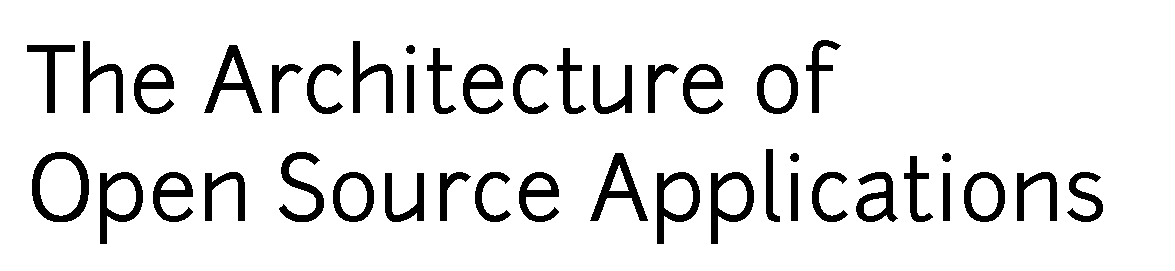
\includegraphics[width=400pt]{../images/frontmatter/title.eps} 

\newpage

% Blank page here
\thispagestyle{empty}
\mbox{}    % need to have *something* in here or Latex "helpfully" removes page

\newpage
% title page

\thispagestyle{empty}
\hspace{-2cm}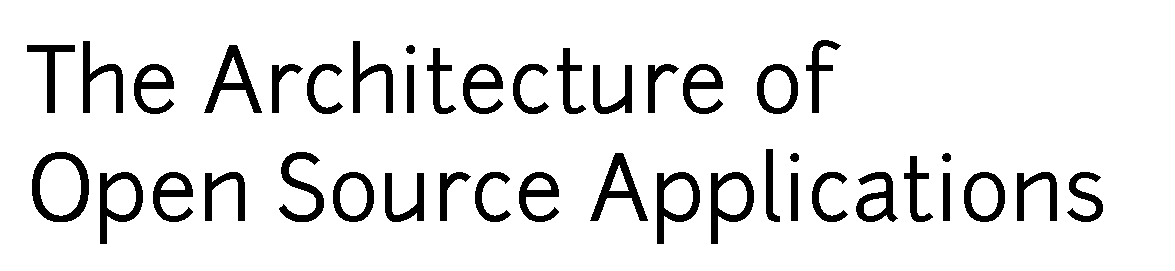
\includegraphics[width=400pt]{../images/frontmatter/title.eps} 
\\
\vspace{0.5cm}
\hspace{2.8cm}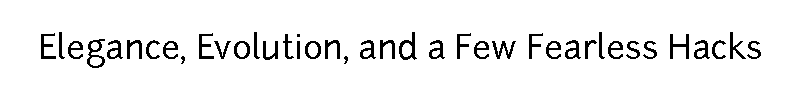
\includegraphics{../images/frontmatter/subtitle.eps}
\\[13.5cm]
\vspace{0.5cm}
\hspace{6.5cm}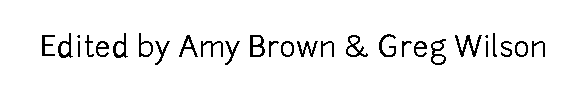
\includegraphics{../images/frontmatter/eds.eps}

\newpage
% copyright page 

\thispagestyle{empty}

\small
%% \noindent \textbf{The Architecture of Open Source Applications} \\
%% Edited by Amy Brown and Greg Wilson
\noindent \textbf{オープンソースアプリケーションのアーキテクチャ} \\
編集:Amy Brown and Greg Wilson \\
翻訳:Arai Kunimitsu and TAKAGI Masahiro

\vspace{0.15cm}

\noindent
%% This work is licensed under the Creative Commons Attribution 3.0
%% Unported license (CC~BY~3.0).  You are free:
この日本語訳はCreative Commons表示3.0非移植ライセンス(CC~BY~3.0)のもとで公開します。あなたは以下の条件に従う限り、自由に

\begin{aosaitemize}
  %% \item to Share---to copy, distribute and transmit the work
  %% \item to Remix---to adapt the work
  \item 本作品を複製、頒布、展示、実演することができます。
  \item 二次的著作物を作成することができます。
  \item 本作品を営利目的で利用することができます。
\end{aosaitemize}

\noindent
%% under the following conditions:
あなたが従うべき条件は以下の通りです。

\begin{aosaitemize}
  %% \item Attribution---you must attribute the work in the manner
  %%   specified by the author or licensor (but not in any way that
  %%   suggests that they endorse you or your use of the work).
  \item 表示---あなたは原著作者のクレジットを表示しなければなりません。
\end{aosaitemize}

\noindent
%% with the understanding that:
以下のような理解に基づいています。

\begin{aosaitemize}

  %% \item Waiver---Any of the above conditions can be waived if you get
  %%   permission from the copyright holder.
  \item 放棄---この作品について著作権者等の権利者から別途許可を得た場合は、上記の許諾条件は適用されません。

  %% \item Public Domain---Where the work or any of its elements is in
  %%   the public domain under applicable law, that status is in no way
  %%   affected by the license.
  \item パブリック・ドメイン---作品やその要素が、適用される法律の下でパブリックドメインに属する場合、その状態がこのライセンスによって影響されることはありません。

  %% \item Other Rights---In no way are any of the following rights
  %%   affected by the license:
  \item そのほかの諸権利---ライセンスによって、以下の諸権利が影響を受けるということは全くありません。
    \begin{aosaitemize}

      %% \item Your fair dealing or fair use rights, or other applicable
      %%   copyright exceptions and limitations;
      \item あなたのフェア・ディーリングやフェア・ユースの権利、そのほか著作権の例外・制限規定

      %% \item The author's moral rights;
      \item 著作者人格権

      %% \item Rights other persons may have either in the work itself or
      %%   in how the work is used, such as publicity or privacy rights.
      \item 他の人がこの作品あるいはその使われ方に関して持つ可能性のある権利、たとえばパブリシティ権やプライバシー権

    \end{aosaitemize}

  %% \item Notice---For any reuse or distribution, you must make clear to
  %%   others the license terms of this work. The best way to do this is
  %%   with a link to \url{http://creativecommons.org/licenses/by/3.0/}.
  \item Notice---再利用や頒布にあたっては、この作品の使用許諾条件を他の人々に明らかにしなければなりません。一番よい方法は、\url{http://creativecommons.org/licenses/by/3.0/}へのリンクを示すことです。

\end{aosaitemize}

%% \noindent To view a copy of this license, visit
%% \url{http://creativecommons.org/licenses/by/3.0/} or send a letter to Creative
%% Commons, 444 Castro Street, Suite 900, Mountain View, California,
%% 94041, USA.\\
\noindent このライセンスのコピーを見るには、
\url{http://creativecommons.org/licenses/by/3.0/}を見るか、手紙をCreative
Commons, 444 Castro Street, Suite 900, Mountain View, California,
94041, USA.に送ってください。\\

\vspace{0.15cm}

\noindent
%% The full text of this book is available online at \url{http://www.aosabook.org/}.\\
%% All royalties from its sale will be donated to Amnesty International.\\
本書の全文は、\url{http://www.aosabook.org/}でオンラインで読めます。\\
(英語版の)印税はすべて、アムネスティ・インターナショナルに寄付されます。\\

\vfill

%% \noindent Product and company names mentioned herein may be the trademarks of
%% their respective owners.\\
\noindent 本書に記載されている製品名や会社名は、各社の登録商標あるいは商標である可能性があります。\\

\vspace{0.15cm}

%% \noindent While every precaution has been taken in the preparation of this
%% book, the editors and authors assume no responsibility for errors or omissions,
%% or for damages resulting from the use of the information contained herein.\\
\noindent 本書の製作にあたっては十分に注意を払いましたが、編集者や執筆者そして翻訳者は本書の内容についてなんらかの保証をするものではなく、その内容に基づくいかなる被害に関しても一切の責任を負いません。\\

\vspace{0.15cm}

%% \noindent The cover image is a photograph by Peter Dutton. The photograph is
%% licensed under the Creative Commons Attribution-NonCommercial-ShareAlike 2.0
%% Generic license. To view a copy of this license, visit
%% \url{http://creativecommons.org/licenses/by-nc-sa/2.0/} or send a letter to
%% CreativeCommons, 444 Castro Street, Suite 900, Mountain View, California,
%% 94041, USA. \\
\noindent 表紙の画像はPeter Duttonが撮影した写真です。この写真はCreative Commons表示 - 非営利 - 継承 2.0 一般でライセンスされています。このライセンスのコピーを見るには、
\url{http://creativecommons.org/licenses/by-nc-sa/2.0/}を見るか、手紙を
CreativeCommons, 444 Castro Street, Suite 900, Mountain View, California,
94041, USA.に送ってください。\\

\vspace{1cm}

\noindent Revision Date: \today \\

%% \noindent ISBN: 978-1-257-63801-7
\normalsize

\newpage
% Dedication page

\thispagestyle{empty}

\vspace*{5cm}
\begin{center}
%% \hspace{0cm}Dedicated to Brian Kernighan,\\
%% who has taught us all so much;\\
%% and to prisoners of conscience everywhere.
\hspace{0cm}我々にすべてを教えてくれたBrian Kernighanに\\
そして世界中にいる良心の囚人たちに
\end{center}

\newpage

% Blank page here
\thispagestyle{empty}
\mbox{}    % need to have *something* in here or Latex "helpfully" removes page

